%package list
\documentclass{article}
\usepackage[top=3cm, bottom=3cm, outer=3cm, inner=3cm]{geometry}
\usepackage{multicol}
\usepackage{graphicx}
\usepackage{url}
%\usepackage{cite}
\usepackage{hyperref}
\usepackage{array}
%\usepackage{multicol}
\newcolumntype{x}[1]{>{\centering\arraybackslash\hspace{0pt}}p{#1}}
\usepackage{natbib}
\usepackage{pdfpages}
\usepackage{multirow}
\usepackage[normalem]{ulem}
\useunder{\uline}{\ul}{}
\usepackage{svg}
\usepackage{xcolor}
\usepackage{listings}
\lstdefinestyle{ascii-tree}{
    literate={├}{|}1 {─}{--}1 {└}{+}1 
  }
\lstset{basicstyle=\ttfamily,
  showstringspaces=false,
  commentstyle=\color{red},
  keywordstyle=\color{blue}
}
%\usepackage{booktabs}
\usepackage{caption}
\usepackage{subcaption}
\usepackage{float}
\usepackage{array}

\newcolumntype{M}[1]{>{\centering\arraybackslash}m{#1}}
\newcolumntype{N}{@{}m{0pt}@{}}


%%%%%%%%%%%%%%%%%%%%%%%%%%%%%%%%%%%%%%%%%%%%%%%%%%%%%%%%%%%%%%%%%%%%%%%%%%%%
%%%%%%%%%%%%%%%%%%%%%%%%%%%%%%%%%%%%%%%%%%%%%%%%%%%%%%%%%%%%%%%%%%%%%%%%%%%%
\newcommand{\itemEmail}{rvaldiviase@unsa.edu.pe}
\newcommand{\itemStudent}{Ryan Fabian Valdivia Segovia}
\newcommand{\itemCourse}{Fundamentos de la programación 2}
\newcommand{\itemCourseCode}{1701213}
\newcommand{\itemSemester}{II}
\newcommand{\itemUniversity}{Universidad Nacional de San Agustín de Arequipa}
\newcommand{\itemFaculty}{Facultad de Ingeniería de Producción y Servicios}
\newcommand{\itemDepartment}{Departamento Académico de Ingeniería de Sistemas e Informática}
\newcommand{\itemSchool}{Escuela Profesional de Ingeniería de Sistemas}
\newcommand{\itemAcademic}{2023 - B}
\newcommand{\itemInput}{Del 11 de Octubre 2023}
\newcommand{\itemOutput}{Al 16 de Octubre 2023}
\newcommand{\itemPracticeNumber}{08}
\newcommand{\itemTheme}{HashMap}
%%%%%%%%%%%%%%%%%%%%%%%%%%%%%%%%%%%%%%%%%%%%%%%%%%%%%%%%%%%%%%%%%%%%%%%%%%%%
%%%%%%%%%%%%%%%%%%%%%%%%%%%%%%%%%%%%%%%%%%%%%%%%%%%%%%%%%%%%%%%%%%%%%%%%%%%%

\usepackage[english,spanish]{babel}
\usepackage[utf8]{inputenc}
\AtBeginDocument{\selectlanguage{spanish}}
\renewcommand{\figurename}{Figura}
\renewcommand{\refname}{Referencias}
\renewcommand{\tablename}{Tabla} %esto no funciona cuando se usa babel
\AtBeginDocument{%
	\renewcommand\tablename{Tabla}
}

\usepackage{fancyhdr}
\pagestyle{fancy}
\fancyhf{}
\setlength{\headheight}{30pt}
\renewcommand{\headrulewidth}{1pt}
\renewcommand{\footrulewidth}{1pt}
\fancyhead[L]{\raisebox{-0.2\height}{
\includegraphics[width=3cm]{img/logo_episunsa.png}}}
\fancyhead[C]{\fontsize{7}{7}\selectfont	\itemUniversity \\ \itemFaculty \\ \itemDepartment \\ \itemSchool \\ \textbf{\itemCourse}}
\fancyhead[R]{\raisebox{-0.2\height}{
\includegraphics[width=1.2cm]{img/logo_abet}}}
\fancyfoot[L]{Estudiante Ryan Valdivia}
\fancyfoot[C]{\itemCourse}
\fancyfoot[R]{Página \thepage}

% para el codigo fuente
\usepackage{listings}
\usepackage{color, colortbl}
\definecolor{dkgreen}{rgb}{0,0.6,0}
\definecolor{gray}{rgb}{0.5,0.5,0.5}
\definecolor{mauve}{rgb}{0.58,0,0.82}
\definecolor{codebackground}{rgb}{0.95, 0.95, 0.92}
\definecolor{tablebackground}{rgb}{0.8, 0, 0}

\lstset{frame=tb,
	language=bash,
	aboveskip=3mm,
	belowskip=3mm,
	showstringspaces=false,
	columns=flexible,
	basicstyle={\small\ttfamily},
	numbers=none,
	numberstyle=\tiny\color{gray},
	keywordstyle=\color{blue},
	commentstyle=\color{dkgreen},
	stringstyle=\color{mauve},
	breaklines=true,
	breakatwhitespace=true,
	tabsize=3,
	backgroundcolor= \color{codebackground},
}

\begin{document}
	
	\vspace*{10px}
	
	\begin{center}	
		\fontsize{17}{17} \textbf{ Informe de Laboratorio \itemPracticeNumber}
	\end{center}
	\centerline{\textbf{\Large Tema: \itemTheme}}
	%\vspace*{0.5cm}	

	\begin{flushright}
		\begin{tabular}{|M{2.5cm}|N|}
			\hline 
			\rowcolor{tablebackground}
			\color{white} \textbf{Nota}  \\
			\hline 
			     \\[30pt]
			\hline 			
		\end{tabular}
	\end{flushright}	

	\begin{table}[H]
		\begin{tabular}{|x{4.7cm}|x{4.8cm}|x{4.8cm}|}
			\hline 
			\rowcolor{tablebackground}
			\color{white} \textbf{Estudiante} & \color{white}\textbf{Escuela}  & \color{white}\textbf{Asignatura}   \\
			\hline 
			{\itemStudent \par \itemEmail} & \itemSchool & {\itemCourse \par Semestre: \itemSemester \par Código: \itemCourseCode}     \\
			\hline 			
		\end{tabular}
	\end{table}		
	
	\begin{table}[H]
		\begin{tabular}{|x{4.7cm}|x{4.8cm}|x{4.8cm}|}
			\hline 
			\rowcolor{tablebackground}
			\color{white}\textbf{Laboratorio} & \color{white}\textbf{Tema}  & \color{white}\textbf{Duración}   \\
			\hline 
			\itemPracticeNumber & \itemTheme & 04 horas   \\
			\hline 
		\end{tabular}
	\end{table}
	
	\begin{table}[H]
		\begin{tabular}{|x{4.7cm}|x{4.8cm}|x{4.8cm}|}
			\hline 
			\rowcolor{tablebackground}
			\color{white}\textbf{Semestre académico} & \color{white}\textbf{Fecha de inicio}  & \color{white}\textbf{Fecha de entrega}   \\
			\hline 
			\itemAcademic & \itemInput &  \itemOutput  \\
			\hline 
		\end{tabular}
	\end{table}
	
	\section{Tarea}
	\begin{itemize}
		\subsection{Videojuego}
			\item Cree un Proyecto llamado Laboratorio8
			\item Usted deberá crear las dos clases Soldado.java y VideoJuego5.java. Puede reutilizar lo
desarrollado en Laboratorios anteriores.
			\item Del Soldado nos importa el nombre, puntos de vida, fila y columna (posición en el tablero).
			\item El juego se desarrollará en el mismo tablero de los laboratorios anteriores. Para crear el
tablero utilice la estructura de datos más adecuada.
			\item Tendrá 2 Ejércitos (usar HashMaps). Inicializar el tablero con n soldados aleatorios entre 1 y
10 para cada Ejército. Cada soldado tendrá un nombre autogenerado: Soldado0X1,
Soldado1X1, etc., un valor de puntos de vida autogenerado aleatoriamente [1..5], la fila y
columna también autogenerados aleatoriamente (no puede haber 2 soldados en el mismo
cuadrado). Se debe mostrar el tablero con todos los soldados creados (distinguir los de un
ejército de los del otro ejército). Además de los datos del Soldado con mayor vida de cada
ejército, el promedio de puntos de vida de todos los soldados creados por ejército, los datos
de todos los soldados por ejército en el orden que fueron creados y un ranking de poder de
todos los soldados creados por ejército (del que tiene más nivel de vida al que tiene menos)
usando 2 diferentes algoritmos de ordenamiento (indicar conclusiones respecto a este ordenamiento de HashMaps). Finalmente, que muestre qué ejército ganará la batalla (indicar
la métrica usada para decidir al ganador de la batalla). Hacerlo como programa iterativo.
	\end{itemize}
		
	\section{Equipos, materiales y temas utilizados}
	\begin{itemize}
		\item Sistema Operativo Windows 11 Home Single Language 64 bits 22621.2283
		\item VIM 9.0.
		\item Visual Studio Code 64 bits 1.82.2
		\item OpenJDK 64-Bits 11.0.16.1
		\item Git 2.41.0.windows.1
		\item Cuenta en GitHub con el correo institucional. 
	\end{itemize}
	
	\section{URL de Repositorio Github}
	\begin{itemize}
		\item URL del Repositorio GitHub para clonar o recuperar.
		\item \url{https://github.com/RyanValdivia/fp2-23b.git}
		\item URL para el laboratorio 08 en el Repositorio GitHub.
		\item \url{https://github.com/RyanValdivia/fp2-23b/tree/main/fase02/lab08}
	\end{itemize}
	
	\section{Actividades}
	\subsection{Actividad 1}
	
	\begin{itemize}	
		\item En primer lugar, realicé un commit conteniendo el código de la clase Soldado.java, requerido para la clase principal
	\end{itemize}	
	\begin{lstlisting}[language=bash,caption={Obteniendo la clase Soldado}][H]
		$ git log lab06
		commit 23a84e524fbe434a9e2a93ac1faac82caf5c5298
		Author: RYAN VALDIVIA <rvaldiviase@unsa.edu.pe>
		Date:   Sun Oct 22 14:22:03 2023 -0500
			Version casi final del codigo, puliendo la eficiencia y reciclando el codigo de laboratorios pasados, pero adaptandolos a mapas
	\end{lstlisting}
	\begin{itemize}	
		\item Conteniendo el siguiente código
	\end{itemize}
	\begin{lstlisting}[language=java,caption={Clase Soldado}, numbers=left][H]
public class Soldado {
    private String nombre;
    private int vida;
    private int fila;
    private int columna;
    private String bandera;

    public void setNombre(String s) {
        this.nombre = s;
    }

    public void setVida(int n) {
        this.vida = n;
    }

    public void setFila(int n) {
        this.fila = n;
    }

    public void setColumna(int n) {
        this.columna = n;
    }

    public void setBandera(String s) {
        this.bandera = s;
    }

    public String getNombre() {
        return nombre;
    }

    public int getVida() {
        return vida;
    }

    public int getFila() {
        return fila;
    }

    public int getColumna() {
        return columna;
    }

    public String getBandera() {
        return bandera;
    }
}

	\end{lstlisting}
	\begin{itemize}	
		\item Para este problema, reutilicé el código del anterior laboratorio para contener el talero, ya que me daban libertad de elegir la estructura de datos que quiera para el tablero, así que usaré un arreglo bidimensional.
	\end{itemize}
	\begin{lstlisting}[language=java,caption={Código parcial reciclado}, numbers=left][H]
	public static void main(String[] args) {
        Scanner sc = new Scanner(System.in);
        do {
            Soldado[][] tablero = new Soldado[10][10];
            int ej1 = (int) (Math.random() * 10 + 1);
            int ej2 = (int) (Math.random() * 10 + 1);

            HashMap<String, Soldado> ejercito1 = new HashMap<>();
            HashMap<String, Soldado> ejercito2 = new HashMap<>();

            int[] filas1 = numerosRandom(ej1);
            int[] columnas1 = numerosRandom(ej1);
            int[] filas2;
            int[] columnas2;
            do {
                filas2 = numerosRandom(ej2);
                columnas2 = numerosRandom(ej2);
            } while (!diffCoordenadas(filas1, filas2, columnas1, columnas2));
    
    public static int[] numerosRandom(int q) {
        int[] nums = new int[q];
        for (int i = 0; i < nums.length; i++) {
            nums[i] = nums.length;
        }
        for (int i = 0; i < q; i++) {
            int n;
            do {
                n = (int) (Math.random() * 10);
            } while (estaEnArreglo(nums, n, i));
            nums[i] = n;
        }
        return nums;
    }

    public static boolean estaEnArreglo(int[] arreglo, int num, int indice) {
        for (int i = 0; i < indice; i++) {
            if (arreglo[i] == num) {
                return true;
            }
        }
        return false;
    }

    public static boolean diffCoordenadas(int[] filas1, int[] filas2, int[] columnas1, int[] columnas2) {
        if (filas1.length > filas2.length) {
            for (int i = 0; i < filas2.length; i++) {
                if (filas1[i] == filas2[i] && columnas1[i] == columnas2[i]) {
                    return false;
                }
            }
        } else {
            for (int i = 0; i < filas1.length; i++) {
                if (filas1[i] == filas2[i] && columnas1[i] == columnas2[i]) {
                    return false;
                }
            }
        }
        return true;
    }
	\end{lstlisting}
	\begin{itemize}	
		\item Solo que, en este caso, los dos ejércitos serán almacenados en dos HashMap, por lo que hay que cambiar de estrategia al momento de inicializar los ejércitos, recorriendo los arreglos de coordenadas y asignando los valores al mapa, utilizando los nombres de los Soldados como claves y los objetos como tal como valores.
	\end{itemize}
	\begin{lstlisting}[language=java,caption={Inicializar mapa}, numbers=left][H]
		inicializarEjercito(ejercito1, filas1, columnas1, 1);
        inicializarEjercito(ejercito2, filas2, columnas2, 2);
            
	public static void inicializarEjercito(HashMap<String, Soldado> army, int[] x, int[] y, int ej) {
        for (int i = 0; i < x.length; i++) {
            String key = "Soldado" + i + "X" + ej;
            int v = (int) (Math.random() * 5 + 1);
            army.put(key, new Soldado());
            army.get(key).setNombre(key);
            army.get(key).setFila(x[i]);
            army.get(key).setColumna(y[i]);
            army.get(key).setVida(v);
            if (ej == 1) {
                army.get(key).setBandera("##########");
            } else {
                army.get(key).setBandera("**********");
            }
        }
    }
    
	\end{lstlisting}
	\begin{itemize}	
		\item Una vez inicializados los mapas que contendrán a todos los soldados, debía desplegarlos en el tablero, para esto, primero debía inicializar el tablero, como en el laboratorio anterior, por lo que reciclé código.
	\end{itemize}
	\begin{lstlisting}[language=java,caption={Inicializar tablero}, numbers=left][H]
	public static void inicializarTablero(Soldado[][] tb) {
        for (int i = 0; i < tb.length; i++) {
            for (int j = 0; j < tb[i].length; j++) {
                tb[i][j] = new Soldado();
                tb[i][j].setNombre("          ");
                tb[i][j].setBandera("          ");
            }
        }
    }
	\end{lstlisting}	
	\begin{itemize}	
		\item Una vez inicializado el tablero, viene lo interesante, desplegar a los ejércitos, para ello, recorrí los mapas y asigné los Soldados a sus respectivas posiciones basándome en sus atributos de fila y columna, usando una función lambda con el método 'forEach()' de la clase HashMap.
	\end{itemize}
	\begin{lstlisting}[language=java,caption={Desplegando a los soldados}, numbers=left][H]
		desplegarEjercito(tablero, ejercito1);
		desplegarEjercito(tablero, ejercito2);
	 public static void desplegarEjercito(Soldado[][] tb, HashMap<String, Soldado> army) {
        army.forEach((key, value) -> {
            tb[value.getFila()][value.getColumna()] = value;
        });
    }
	\end{lstlisting}
	\begin{itemize}	
		\item Una vez ya desplegados, quedaba mostrar el tablero, lo cual fue sencillo, ya que reutilicé el código del anterior laboratorio.
	\end{itemize}
	\begin{lstlisting}[language=java,caption={Mostrando el tablero}, numbers=left][H]
	 public static void mostrarTablero(Soldado[][] tb) {
        String vacio = "          ";
        System.out.println(crearTecho());
        for (int i = 0; i < tb.length; i++) {
            System.out.println(separadorSup());
            for (int j = 0; j < tb[i].length; j++) {
                if (j == tb[i].length - 1) {
                    System.out.print("| " + tb[i][j].getBandera() + " |\n");
                } else {
                    System.out.print("| " + tb[i][j].getBandera() + " ");
                }
            }
            for (int j = 0; j < tb[i].length; j++) {
                if (j == tb[i].length - 1) {
                    System.out.print("| " + tb[i][j].getNombre() + " |\n");
                } else {
                    System.out.print("| " + tb[i][j].getNombre() + " ");
                }
            }
            for (int j = 0; j < tb[i].length; j++) {
                if (tb[i][j].getVida() != 0) {
                    if (j == tb[i].length - 1) {
                        System.out.print("|    " + tb[i][j].getVida() + " HP" + "    |\n");
                    } else {
                        System.out.print("|    " + tb[i][j].getVida() + " HP" + "    ");
                    }
                } else {
                    if (j == tb[i].length - 1) {
                        System.out.print("| " + vacio + " |\n");
                    } else {
                        System.out.print("| " + vacio + " ");
                    }
                }
            }
            System.out.println(separadorInf());
        }
        System.out.println();
    }
	\end{lstlisting}

	
	\begin{itemize}
		\item Imprimiendo esto al momento de ejecutar el código.
	\end{itemize}
	
	\begin{figure}[H]
		\centering
	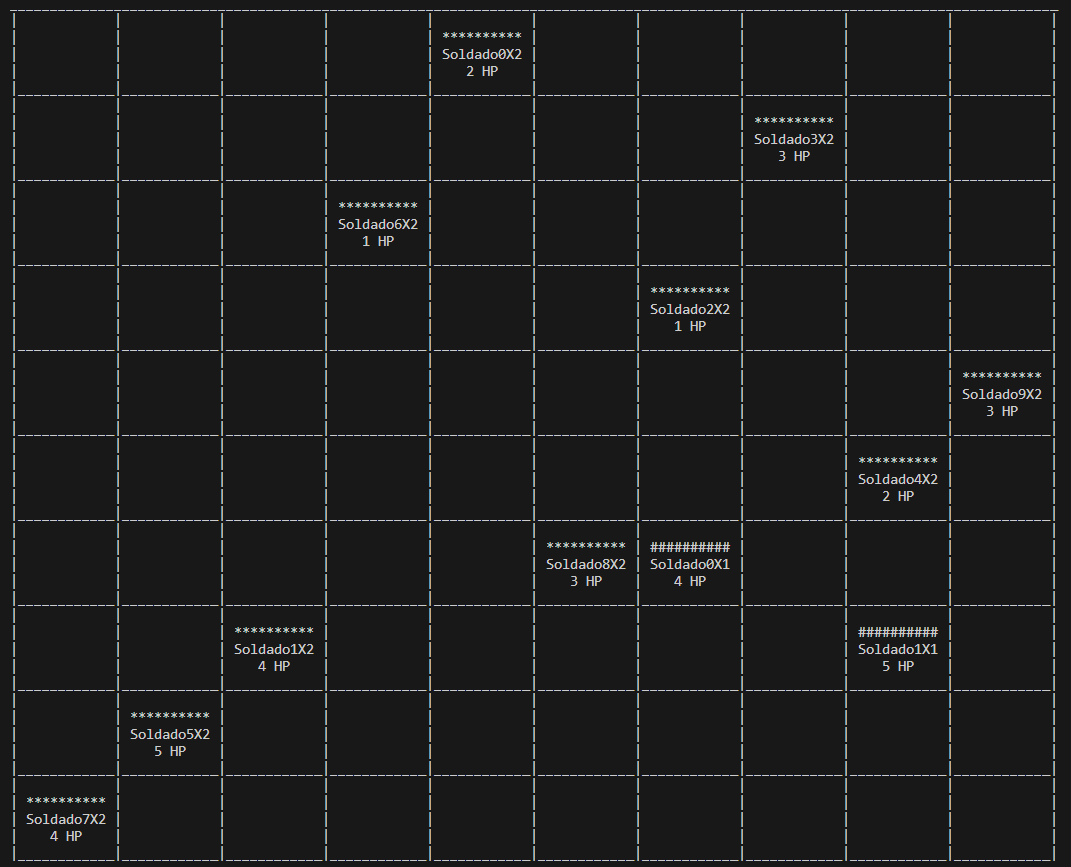
\includegraphics[width=0.8\textwidth,keepaspectratio]{img/captura1.png}
		%\includesvg{img/automata.svg}
		%\label{img:mot2}
		%\caption{Product backlog.}
	\end{figure}
	
	\begin{itemize}	
		\item Una vez terminado el tablero, pasé a trabajar el resto de requerimientos para el programa.
		\item Ahora debía mostrar el soldado con mayor nivel de vida, para esto, solo debía recorrer el mapa buscando el soldado con mayor vida, tomando el primer valor del mapa como pivote y comprar cada entrada para ver si es mayor o no, una vez encontrado el soldado con mayor vida, se muestra usando otro método reutilizado.
	\end{itemize}
	\begin{lstlisting}[language=java,caption={Soldado con mayor vida}, numbers=left][H]
			soldadoMayorVida(ejercito1, 1);
			soldadoMayorVida(ejercito2, 2);
			
	  public static void soldadoMayorVida(Map<String, Soldado> army, int ej) {
        boolean pro = true;
        String keyMx = "";
        for (Map.Entry<String, Soldado> entry : army.entrySet()) {
            if (pro) {
                keyMx = entry.getKey();
                pro = false;
            }
            if (army.get(keyMx).getVida() < entry.getValue().getVida()) {
                keyMx = entry.getKey();
            }
        }
        System.out.println("El soldado con mayor vida del ejercito " + ej + " es: ");
        mostrarSoldado(army.get(keyMx));
        System.out.println();

    }
    public static void mostrarSoldado(Soldado s) {
        String columna;
        System.out.println("Nombre: " + s.getNombre());
        System.out.println("Vida: " + s.getVida() + " HP");
        switch (s.getColumna() + 1) {
            case 1:
                columna = "A";
                break;
            case 2:
                columna = "B";
                break;
            case 3:
                columna = "C";
                break;
            case 4:
                columna = "D";
                break;
            case 5:
                columna = "E";
                break;
            case 6:
                columna = "F";
                break;
            case 7:
                columna = "G";
                break;
            case 8:
                columna = "H";
                break;
            case 9:
                columna = "I";
                break;
            case 10:
                columna = "J";
                break;
            default:
                columna = "K";
                break;
        }
        System.out.println("Posicion: " + (s.getFila() + 1) + "-" + columna);
        System.out.println();
    }
	\end{lstlisting}
	\begin{itemize}	
		\item Después, seguía el mostrar la vida total y promedio de cada ejército. Para ello, solo debía recorrer el mapa y sumar la vida de todos los valores.
	\end{itemize}
	\begin{lstlisting}[language=java,caption={Vida promedio y total}, numbers=left][H]
		vidaPromedio(ejercito1, 1);
		vidaPromedio(ejercito2, 2);
	
	public static void vidaPromedio(HashMap<String, Soldado> army, int ej) {
        int total = 0;
        for (Map.Entry<String, Soldado> entry : army.entrySet()) {
            total += entry.getValue().getVida();
        }
        System.out.println("La vida total del ejercito " + ej + " es: " + total);
        System.out.println("La vida promedio del ejercito " + ej + " es: " + total / (1.0 * army.size()));
        System.out.println();
    }
	\end{lstlisting}
	\begin{itemize}	
		\item Mostrando lo siguiente al momento de ejecutar el código (Siguiendo con la ejecución de la anterior captura).
	\end{itemize}
	
	\begin{figure}[H]
		\centering
	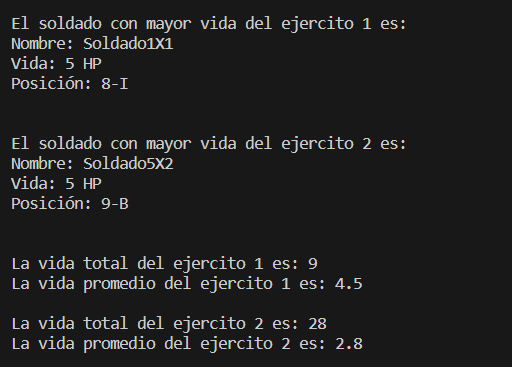
\includegraphics[width=0.8\textwidth,keepaspectratio]{img/captura2.png}
		%\includesvg{img/automata.svg}
		%\label{img:mot2}
		%\caption{Product backlog.}
	\end{figure}
	\begin{itemize}	
		\item Ahora seguía algo más complicado, mostrar el ejército según el orden de creación de los soldados, para esto, no me servía simplemente recorrer el mapa, ya que en HashMap, no se sigue un orden según la inserción, por lo tanto, debía guiarme de otra cosa, como las keys de los objetos (Por eso le puse como claves a los objetos, sus respectivos nombres) dando lugar al siguiente método.
	\end{itemize}
	
	\begin{lstlisting}[language=java,caption={Mostrando el ejército}, numbers=left][H]
	public static void mostrarEjercito(Map<String, Soldado> army, int ej) {
        System.out.println("Ejercito " + ej);
        for (int i = 0; i < army.size(); i++) {
            String key = "Soldado" + i + "X" + ej;
            mostrarSoldado(army.get(key));
        }
        System.out.println();
    }
	\end{lstlisting}
	\begin{itemize}	
		\item Mostrando lo siguiente al momento de ejecutar:
	\end{itemize}
	
	\begin{figure}[H]
		\centering
	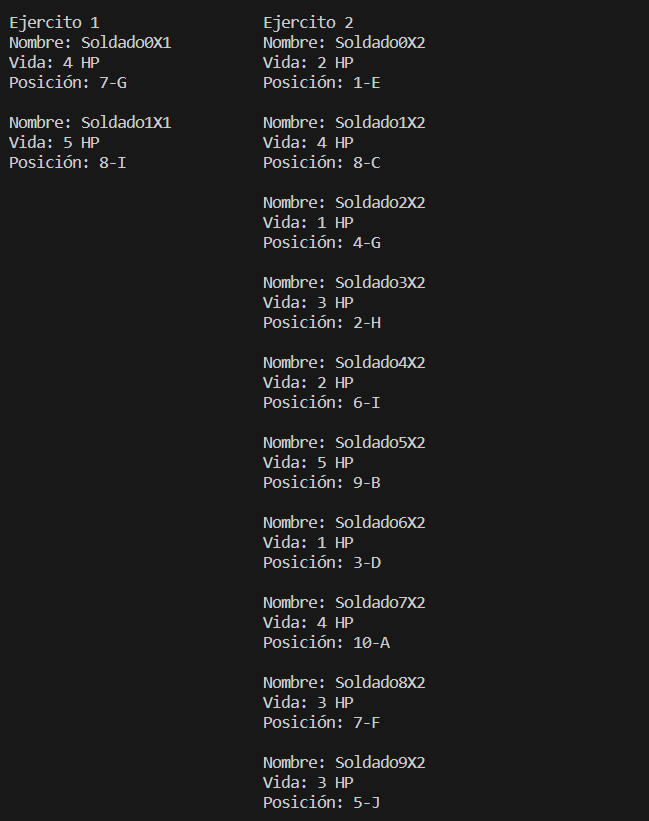
\includegraphics[width=0.8\textwidth,keepaspectratio]{img/captura3.png}
		%\includesvg{img/automata.svg}
		%\label{img:mot2}
		%\caption{Product backlog.}
	\end{figure}
	
	\begin{itemize}	
		\item Ahora sigue algo mucho más difícil, ordenar los mapas y mostrar el Ranking de soldados de mayor a menor vida.
		\item El principal problema es que los HashMap no siguen un orden por inserción, por lo tanto, sería imposible ordenar uno, es por ello que tuve que buscar una alternativa.
		\item Lo primero que hice, fue copiar todos los valores (objetos / Soldados) del mapa, a una lista, para posteriormente ordenarla según el algoritmo deseado. Una vez terminado esto, copiaba de nuevo los objetos ya ordenados a un nuevo mapa, pero ya no un HashMap, sino, un LinkedHashMap, ya que este, a diferencia del normal, si sigue un orden según la inserción.
	\end{itemize}
	
	\begin{lstlisting}[language=java,caption={Algoritmos de ordenamiento}, numbers=left][H]
	 public static LinkedHashMap<String, Soldado> bubbleSort(HashMap<String, Soldado> map, int ej) {
        ArrayList<Soldado> army = getLista(map);
        boolean sorted = false;
        while (!sorted) {
            sorted = true;
            for (int i = 0; i < army.size() - 1; i++) {
                if (army.get(i).getVida() < army.get(i + 1).getVida()) {
                    Soldado temp = army.get(i);
                    army.set(i, army.get(i + 1));
                    army.set(i + 1, temp);
                    sorted = false;
                }
            }
        }
        LinkedHashMap<String, Soldado> sortedMap = new LinkedHashMap<>();
        for (int i = 0; i < army.size(); i++) {
            String key = army.get(i).getNombre();
            sortedMap.put(key, army.get(i));
        }
        return sortedMap;
    }

    public static LinkedHashMap<String, Soldado> insertionSort(HashMap<String, Soldado> map, int ej) {
        ArrayList<Soldado> army = getLista(map);
        int i, j;
        for (i = 1; i < army.size(); i++) {
            Soldado tmp = army.get(i);
            j = i;
            while ((j > 0) && (army.get(j - 1).getVida() < tmp.getVida())) {
                army.set(j, army.get(j - 1));
                j--;
            }
            army.set(j, tmp);
        }
        LinkedHashMap<String, Soldado> sortedMap = new LinkedHashMap<>();
        for (int k = 0; k < army.size(); k++) {
            String key = army.get(k).getNombre();
            sortedMap.put(key, army.get(k));
        }
        return sortedMap;

    }

    public static ArrayList<Soldado> getLista(HashMap<String, Soldado> map) {
        ArrayList<Soldado> list = new ArrayList<Soldado>();
        list.addAll(map.values());
        return list;
    }
	\end{lstlisting}
	\begin{itemize}	
		\item De este modo, obtengo un mapa ya ordenado, donde solo me queda recorrerlo imprimiendo los valores de cada soldado, haciendo un pequeño menú para seleccionar el algoritmo de ordenamiento preferido.
	\end{itemize}
	\begin{lstlisting}[language=java,caption={Mostrar mapa ya ordenado}, numbers=left][H]
	System.out.println("Bajo que algoritmo de ordenamiento le gustaria ordenar su ejercito?");
            System.out.println("1. Ordenamiento por burbuja");
            System.out.println("2. Ordenamiento por insercion\n");
            switch (sc.nextInt()) {
                case 1:
                    System.out.println("Ranking por Vida: \n");
                    mostrarOrdenado(bubbleSort(ejercito1, 1), 1);
                    mostrarOrdenado(bubbleSort(ejercito2, 2), 2);
                    break;
                case 2:
                    System.out.println("Ranking por Vida: \n");
                    mostrarOrdenado(insertionSort(ejercito1, 1), 1);
                    mostrarOrdenado(insertionSort(ejercito2, 2), 2);
                    break;
                default:
            }
	public static void mostrarOrdenado(Map<String, Soldado> map, int ej) {
        System.out.println("Ejercito " + ej);
        System.out.println(map.get("Soldado0X" + ej).getBandera() + "\n");
        for (Map.Entry<String, Soldado> entry : map.entrySet()) {
            mostrarSoldado(entry.getValue());
        }
    	}
	\end{lstlisting}
	
	\begin{itemize}	
		\item Mostrando lo siguiente:
	\end{itemize}
	
	\begin{figure}[H]
		\centering
	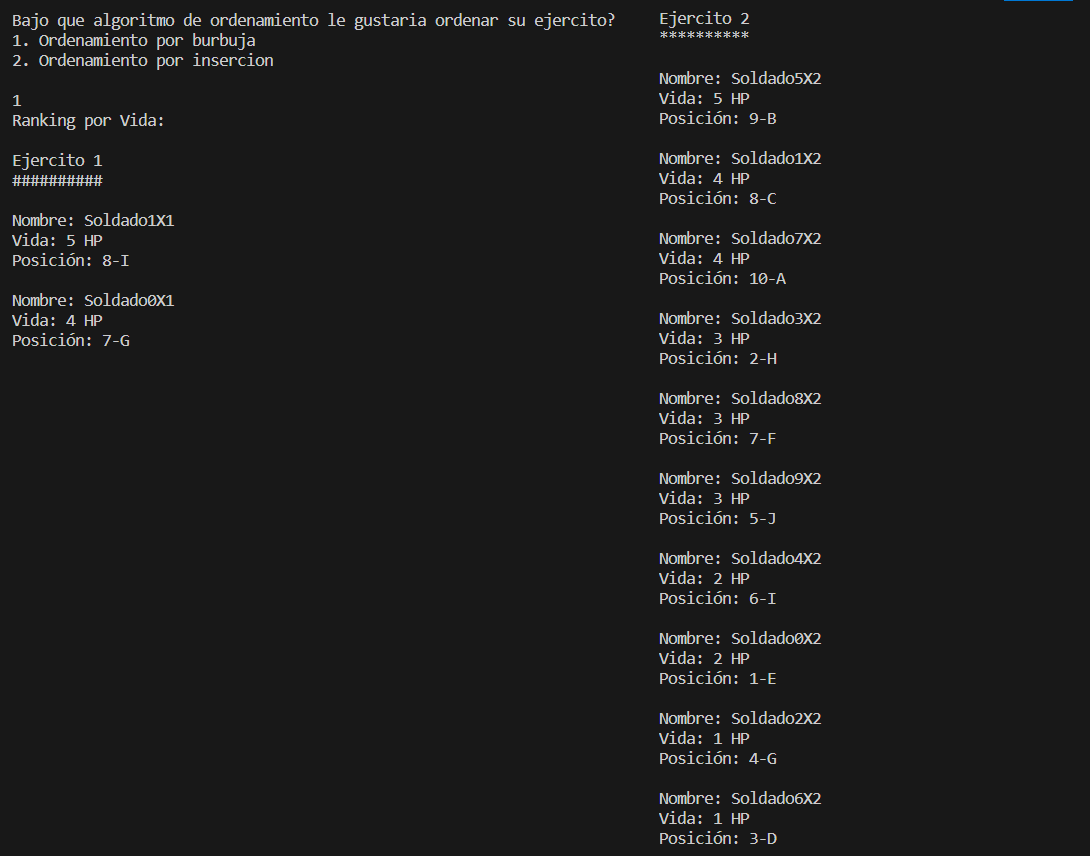
\includegraphics[width=0.6\textwidth,keepaspectratio]{img/captura4.png}
		%\includesvg{img/automata.svg}
		%\label{img:mot2}
		%\caption{Product backlog.}
	\end{figure}
	
	\begin{itemize}	
		\item Una vez culminado esto, solo quedaba algo mucho más simple, determinar cuál ejército gana, para lo cual solo necesitaba comparar los niveles de vida totales de ambos mapas.
		
	\end{itemize}
	\begin{lstlisting}[language=java,caption={Ejército ganador}, numbers=left][H]
	public static void ejercitoGanador(Map<String, Soldado> map1, Map<String, Soldado> map2) {
        int total1 = 0, total2 = 0;
        for (Map.Entry<String, Soldado> entry : map1.entrySet()) {
            total1 += entry.getValue().getVida();
        }
        for (Map.Entry<String, Soldado> entry : map2.entrySet()) {
            total2 += entry.getValue().getVida();
        }
        if (total1 > total2) {
            System.out.println("El ejercito 1 es ganador!");
        } else if (total1 == total2) {
            System.out.println("Hay empate!");
        } else {
            System.out.println("El ejercito 2 es ganador!");
        }
        System.out.println("Bajo la metrica de que ejercito tiene mas vida");
    }
    \end{lstlisting}
	\begin{figure}[H]
		\centering
	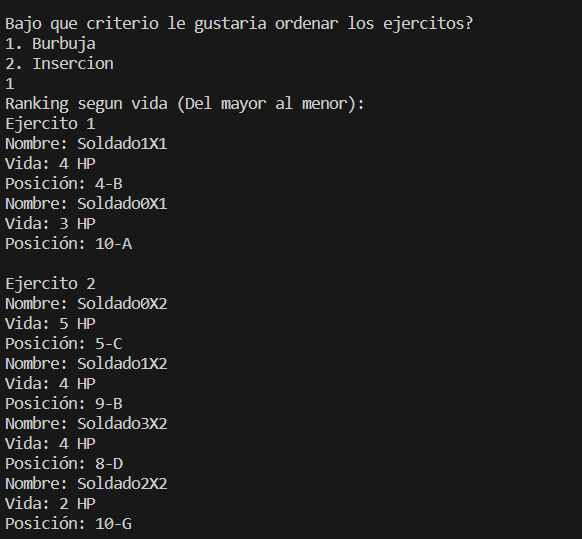
\includegraphics[width=0.6\textwidth,keepaspectratio]{img/captura5.png}
		%\includesvg{img/automata.svg}
		%\label{img:mot2}
		%\caption{Product backlog.}
	\end{figure}
	
	\begin{itemize}	
		\item Ya para terminar, solo faltaría saber qué ejército ganó, para esto, usé el criterio de qué ejército tiene más nivel de vida total.
	\end{itemize}
	
	\begin{lstlisting}[language=java,caption={Determinando el ganador}, numbers=left][H]
	 public static void ejercitoGanador(Soldado[] army1, Soldado[] army2) {
        int total1 = 0;
        int total2 = 0;
        for (int i = 0; i < army1.length; i++) {
            total1 += army1[i].getVida();
        }
        for (int i = 0; i < army2.length; i++) {
            total2 += army2[i].getVida();
        }
        if (total1 > total2) {
            System.out.println("El ejercito 1 es ganador!");
        } else if (total1 == total2) {
            System.out.println("Empate");
        } else {
            System.out.println("El ejercito 2 es ganador");
        }
        System.out.println("Bajo el criterio de que ejercito tiene mas vida total");

    }
	\end{lstlisting}
	\begin{itemize}	
		\item Imprimiendo lo siguiente: 
	\end{itemize}
	
	\begin{figure}[H]
		\centering
	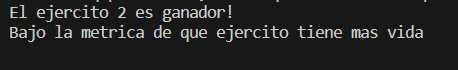
\includegraphics[width=0.5\textwidth,keepaspectratio]{img/captura6.png}
		%\includesvg{img/automata.svg}
		%\label{img:mot2}
		%\caption{Product backlog.}
	\end{figure}
	
	\begin{itemize}	
		\item Y para hacer el programa iterativo, solo coloqué un do-while en el método main, para que se pueda repetir el programa.
	\end{itemize}
	
	\begin{lstlisting}[language=java,caption={Método main final}, numbers=left][H]
	public static void main(String[] args) {
        Scanner sc = new Scanner(System.in);
        do {
            Soldado[][] tablero = new Soldado[10][10];
            int ej1 = (int) (Math.random() * 10 + 1);
            int ej2 = (int) (Math.random() * 10 + 1);

            HashMap<String, Soldado> ejercito1 = new HashMap<>();
            HashMap<String, Soldado> ejercito2 = new HashMap<>();

            int[] filas1 = numerosRandom(ej1);
            int[] columnas1 = numerosRandom(ej1);
            int[] filas2;
            int[] columnas2;
            do {
                filas2 = numerosRandom(ej2);
                columnas2 = numerosRandom(ej2);
            } while (!diffCoordenadas(filas1, filas2, columnas1, columnas2));

            inicializarEjercito(ejercito1, filas1, columnas1, 1);
            inicializarEjercito(ejercito2, filas2, columnas2, 2);
            inicializarTablero(tablero);
            desplegarEjercito(tablero, ejercito1);
            desplegarEjercito(tablero, ejercito2);
            mostrarTablero(tablero);
            soldadoMayorVida(ejercito1, 1);
            soldadoMayorVida(ejercito2, 2);
            vidaPromedio(ejercito1, 1);
            vidaPromedio(ejercito2, 2);
            mostrarEjercito(ejercito1, 1);
            mostrarEjercito(ejercito2, 2);

            System.out.println("Bajo que algoritmo de ordenamiento le gustaria ordenar su ejercito?");
            System.out.println("1. Ordenamiento por burbuja");
            System.out.println("2. Ordenamiento por insercion\n");
            switch (sc.nextInt()) {
                case 1:
                    System.out.println("Ranking por Vida: \n");
                    mostrarOrdenado(bubbleSort(ejercito1, 1), 1);
                    mostrarOrdenado(bubbleSort(ejercito2, 2), 2);
                    break;
                case 2:
                    System.out.println("Ranking por Vida: \n");
                    mostrarOrdenado(insertionSort(ejercito1, 1), 1);
                    mostrarOrdenado(insertionSort(ejercito2, 2), 2);
                    break;
                default:
            }
            System.out.println("Presione q para salir, o cualquier otra tecla para volver a jugar");
            ejercitoGanador(ejercito1, ejercito2);
        } while (!sc.next().equals("q"));

    }
	\end{lstlisting}
	
	
	\section{\textcolor{red}{Rúbricas}}
	
	\subsection{\textcolor{red}{Entregable Informe}}
	\begin{table}[H]
		\caption{Tipo de Informe}
		\setlength{\tabcolsep}{0.5em} % for the horizontal padding
		{\renewcommand{\arraystretch}{1.5}% for the vertical padding
		\begin{tabular}{|p{3cm}|p{12cm}|}
			\hline
			\multicolumn{2}{|c|}{\textbf{\textcolor{red}{Informe}}}  \\
			\hline 
			\textbf{\textcolor{red}{Latex}} & \textcolor{blue}{El informe está en formato PDF desde Latex,  con un formato limpio (buena presentación) y facil de leer.}   \\ 
			\hline 
			
			
		\end{tabular}
	}
	\end{table}
	
	\clearpage
	
	\subsection{\textcolor{red}{Rúbrica para el contenido del Informe y demostración}}
	\begin{itemize}			
		\item El alumno debe marcar o dejar en blanco en celdas de la columna \textbf{Checklist} si cumplio con el ítem correspondiente.
		\item Si un alumno supera la fecha de entrega,  su calificación será sobre la nota mínima aprobada, siempre y cuando cumpla con todos lo items.
		\item El alumno debe autocalificarse en la columna \textbf{Estudiante} de acuerdo a la siguiente tabla:
	
		\begin{table}[ht]
			\caption{Niveles de desempeño}
			\begin{center}
			\begin{tabular}{ccccc}
    			\hline
    			 & \multicolumn{4}{c}{Nivel}\\
    			\cline{1-5}
    			\textbf{Puntos} & Insatisfactorio 25\%& En Proceso 50\% & Satisfactorio 75\% & Sobresaliente 100\%\\
    			\textbf{2.0}&0.5&1.0&1.5&2.0\\
    			\textbf{4.0}&1.0&2.0&3.0&4.0\\
    		\hline
			\end{tabular}
		\end{center}
	\end{table}	
	
	\end{itemize}
	
	\begin{table}[H]
		\caption{Rúbrica para contenido del Informe y demostración}
		\setlength{\tabcolsep}{0.5em} % for the horizontal padding
		{\renewcommand{\arraystretch}{1.5}% for the vertical padding
		%\begin{center}
		\begin{tabular}{|p{2.7cm}|p{7cm}|x{1.3cm}|p{1.2cm}|p{1.5cm}|p{1.1cm}|}
			\hline
    		\multicolumn{2}{|c|}{Contenido y demostración} & Puntos & Checklist & Estudiante & Profesor\\
			\hline
			\textbf{1. GitHub} & Hay enlace URL activo del directorio para el  laboratorio hacia su repositorio GitHub con código fuente terminado y fácil de revisar. &2 &X &2 & \\ 
			\hline
			\textbf{2. Commits} &  Hay capturas de pantalla de los commits más importantes con sus explicaciones detalladas. (El profesor puede preguntar para refrendar calificación). &4 &X &2 & \\ 
			\hline 
			\textbf{3. Código fuente} &  Hay porciones de código fuente importantes con numeración y explicaciones detalladas de sus funciones. &2 &X &2 & \\ 
			\hline 
			\textbf{4. Ejecución} & Se incluyen ejecuciones/pruebas del código fuente  explicadas gradualmente. &2 &X &2 & \\ 
			\hline			
			\textbf{5. Pregunta} & Se responde con completitud a la pregunta formulada en la tarea.  (El profesor puede preguntar para refrendar calificación).  &2 &X &2 & \\ 
			\hline	
			\textbf{6. Fechas} & Las fechas de modificación del código fuente estan dentro de los plazos de fecha de entrega establecidos. &2 &X &2 & \\ 
			\hline 
			\textbf{7. Ortografía} & El documento no muestra errores ortográficos. &2 &X &2 & \\ 
			\hline 
			\textbf{8. Madurez} & El Informe muestra de manera general una evolución de la madurez del código fuente,  explicaciones puntuales pero precisas y un acabado impecable.   (El profesor puede preguntar para refrendar calificación).  &4 &X &4 & \\ 
			\hline
			\multicolumn{2}{|c|}{\textbf{Total}} &20 & &18 & \\ 
			\hline
		\end{tabular}
		%\end{center}
		%\label{tab:multicol}
		}
	\end{table}
	
\clearpage

\section{Referencias}
	\begin{itemize}
		\item Fundamentos de la programación 2 - Tópicos de la programación Orientada a Objetos (Marco Aedo)
	\end{itemize}
	
%\clearpage
%\bibliographystyle{apalike}
%\bibliographystyle{IEEEtranN}
%\bibliography{bibliography}
			
\end{document}
